
\documentclass[10pt,journal,cspaper,compsoc]{IEEEtran}
\hyphenation{op-tical net-works semi-conduc-tor}
\usepackage[pdftex]{graphicx}
\usepackage{url} 

\begin{document}

\title{Price Elasticity of the Enterprise Computing Resource Market}

\author
{
Qingye~Jiang,~\IEEEmembership{Senior Member,~IEEE,}
Young Choon~Lee, 
and~Albert~Y.~Zomaya,~\IEEEmembership{Fellow,~IEEE}%
}


\IEEEcompsoctitleabstractindextext{%
\begin{abstract}
Pricing is an important property of a product in that it significantly affects the customer's purchasing behavior. In the enterprise computing resource market, suppliers often compete for market share with price reductions. In many cases, price reductions are the outcome of business intuition rather than rigorous reasoning, and often at the cost of losing revenue and profit. In this paper, we study the supply and demand relationship of the global enterprise computing resource market, using market research data between 2006 and 2013. The market segments we study include the traditional server sales business, server rental business, and public clouds. We find out that consumers in different market segments are not equally sensitive to price changes. Then we quantitatively measure such sensitivity with the concept of price elasticity of demand. Furthermore, we analyze the success and failure of the major players in the market using the theory of price elasticity of demand. This paper provides new insights into the microeconomics characteristics of the enterprise computing resource market. These findings can help participants in various market segments design better pricing strategies leading to both market diffusion and profitability.
\end{abstract}
\begin{keywords}
enterprise computing resource market, cloud computing, microeconomics, price elasticity of demand
\end{keywords}}

\maketitle
\IEEEdisplaynotcompsoctitleabstractindextext
\IEEEpeerreviewmaketitle

\section{Introduction}
\label{sec:intro}

Pricing strategies are crucial business decisions in the life cycle of a product, especially when there are multiple competitors in the market. In a perfect competition market, there are multiple suppliers offering similar products, while no participant is powerful enough to control the price of the product. To compete for market share, suppliers often use price reduction in promotional campaigns. However, many of such price reductions are the outcome of business intuition rather than rigorous reasoning, and often at the cost of losing revenue and profit.

The enterprise computing resource market seems to be a perfect competition market with multiple players. Traditionally, enterprise can buy servers from hardware vendors, or rent servers from hosting service providers. In recent years, Infrastructure-as-a-Service (IaaS) is gradually making its way into the enterprise computing resource market. As defined by NIST \cite{nist}, IaaS is one of the three service models of cloud computing. It refers to the capability provided to the consumer to provision processing, storage, networking, and other computing resources where the consumer is able to deploy arbitrary software, including operating systems and applications. Within the scope of this paper, the word "cloud computing" refers to IaaS rather than the other two service models. 

Amazon Web Services (AWS) are widely recognized as examples of public cloud services. Over the past years, the market witnessed a trend in developing new applications on AWS, or migrating existing applications to AWS. AWS has become the largest hosting company in the world, as measured by the number of web-facing servers. Cloud computing has clearly demonstrated itself as a revolution in the computing resource market, and has changed the way IT professionals think about the acquisition, provision, and management of computing resource. Inspired by the dramatic growth of AWS, there quickly emerged many followers in the market, including Microsoft Windows Azure, Google Compute Engine, Rackspace, and HP. As new service providers enter the market, they employ price reduction as a strategy to win customers from competitors. In response to such price reductions, existing service providers are forced to carry out further price reductions to maintain competitiveness as evident in the recent AWS 42$^{nd}$ price reduction \cite{web:aws42pricereduction}. Such pricing wars trigger a wide range of discussions. In this study, we are particularly interested in the following three questions. These questions are important in that they represent the relationship between supply and demand, and has a direct impact on a vendor's competitiveness and pricing strategy in the enterprise computing resource market.

\begin{itemize}
	\item Is the enterprise computing resource market a perfect competition market? 
	\item In the enterprise computing resource market, how sensitive the consumers are to price changes?
	\item Is price reduction an effective way to win in the enterprise computing resource market?
\end{itemize}

To answer these questions, we study the supply and demand relationship of the global enterprise computing resource market, using market research data between 2006 and 2013 available from a wide range of data sources  (see Section \ref{sec:data} for details). We quantitatively measure the consumer's sensitivity to price changes using the concept of price elasticity of demand \cite{marshall}. Finally, we analyze the impact of different pricing strategies on the performance of the business in different situations, using the server sales business of IBM, HP and DELL as case studies. This research provides new insights into the microeconomics characteristics of the enterprise computing resource market, and can help participants in various market segments design better pricing strategies leading to both market diffusion and profitability.  

\subsection{Data Sources}
\label{sec:data}
As the amount of data sources used in this study is overwhelming the limited reference list of this paper, we created a dedicated blog entry \cite{qyjohn} hosted on the author's personal blog site, with links to all the data sources. These data sources include Gartner's quarterly reports, Rackspace's annual reports and  the official AWS blog site. They are available in the form of public accessible web pages. 

For the server sales business, we collect data from Gartner's quarterly reports on worldwide server shipments between 2006 and 2013. This report is published on Gartner's website, with the number of server shipments and the revenue generated from server shipments during the previous quarter.  The report also provides break down numbers by hardware vendors, which are analyzed in details in our case studies. For the server rental business, we use Rackspace as an example of this market segment, and collect data regarding revenue and the number of servers from Rackspace's annual report (Form 10-K) to the United States Securities and Exchange Commission (SEC). For public clouds, we use AWS EC2 as an example of this market segment. The pricing history of the AWS EC2 service is collected from the official AWS blog site. However, the actual size (such as the number of physical servers) of AWS has always been part of Amazon's best-kept secrets. In this study, we use the estimated number of servers for EC2 derived by a number of cloud computing professionals in the industry as the foundation to carry out our analysis.

\subsection{Organization}
The rest of this paper is organized as follows. Section \ref{sec:market} describes the three major segments of the enterprise computing resource market. In Section \ref{sec:analysis}, we analyze the price elasticity of demand in those three market segments. Section \ref{sec:casestudies} presents case studies on the impact of different pricing strategies, using IBM, HP and DELL as examples. We review and discuss related work in Section \ref{sec:relatedwork} followed by our conclusions in Section \ref{sec:conclusions}.

\begin{table*}[t]
\caption{Different Segments in the Enterprise Computing Resource Market}
\label{tbl:resourcemarket}
%\begin{center}
\centering
\begin{tabular}{|p{3cm}|p{3cm}|p{3cm}|p{3cm}|}
\hline
 Market segment& Server Sales Business & Server Rental Business & Public Clouds \\ \hline
Major vendors & IBM, HP, DELL, \newline Fujitsu, Oracle & Rackspace, OVH, \newline SoftLayer & Amazon, Rackspace, \newline Microsoft, Google \newline HP \\ \hline
Acquisition time & weeks & days & minutes  \\ \hline
Expense type & CapEx & OpEx & OpEx \\ \hline
Unit cost  & 2,000\~{}50,000 USD\newline one time payment  & 100\~{}2000 USD\newline monthly charge & 0.02\~{}6.82 USD\newline hourly charge \\ \hline
Ownership & consumer & supplier & supplier \\ \hline
Operations & consumer & supplier & supplier \\ \hline
Life cycle & 3 to 5 years & 1 to 36 months & hourly \\ \hline
Contracts & optional service contract & long term contract with SLA & SLA \\ \hline
Market size \newline (number of servers)& 10 million annually \newline 40 million total & 2 million total & 1 million total \\ \hline
Market share & 93\% & 5\% & 2\% \\ \hline
Market growth & linear & linear & exponential \\ \hline
\end{tabular}
%\end{center}
\end{table*}

\section{The Enterprise Computing Resource Market}
\label{sec:market}

As of today, enterprises have three major options to acquire computing resources. They can either buy new servers from hardware vendors, lease servers from hosting service providers, or using public clouds. The different ways to acquire computing resources represent different segments of the enterprise computing resource market, namely server sales business, server rental business, and public clouds (Table \ref{tbl:resourcemarket}). Each of these market segments consists of different suppliers. Furthermore,  they have different business processes, with different financial and human resource requirements for the consumer, as well as other implications such as ownership and contractual liabilities. 

\subsection{Server Sales Business}
The major suppliers in the server sales business are hardware vendors, including IBM, HP, and DELL. Consumers can order servers directly from the vendors, or through a third-party distributor. The cost to acquire new servers is denoted as capital expense (CapEx) in accounting, and is usually paid to the supplier in a single payment before or after hardware delivery. Depending on the brand name and the configuration of the product, the acquisition cost can vary from thousands to tens of thousands of US Dollars per server. The acquisition time (the time needed to deliver the server hardware to the consumer after ordering) usually falls within weeks for low-end servers when local stockage is available, but can be months for high-end servers requiring pre-orders. When the servers are delivered to the consumer, their ownership is also transferred from the supplier to the consumer, and they become fixed-asset of the consumer. The life cycle of server hardware usually falls between three to five years \cite{Greenberg2008}, depending on the accounting and fixed-asset depreciation policies of the consumer. It is the consumer's responsibility to maintain the health of the server hardware, unless the consumer chooses to purchase additional service contracts from the vendor.

According to Gartner’s quarterly reports on worldwide server shipments, 8 to 10 million new servers were shipped to the market on an annual base between 2006 and 2013. Considering the fact that the life cycle of server hardware typically falls between 3 to 5 years, we estimate that there are approximately 40 million servers running worldwide. 

\subsection{Server Rental Business}
The major suppliers in the server rental business are hosting service providers, including Rackspace, OVH, and SoftLayer. Consumers usually establish a server rental contract directly with the service provider. The length of the contract varies from months to years, depending on the consumer's need for computing resource. According to the contract, the consumer pays a recurring monthly fee to maintain access to designated computing resource through network. Such cost is denoted as operations expense (OpEx) in accounting. Depending on the configuration of the computing resource, the recurring cost can vary from hundreds to thousands of US Dollars per server per month. The acquisition time (the time needed to acquire access to computing resource after signing the contract) usually falls within days, but can be weeks if new computing resource needs to be ordered by the service provider. The server rental contract does not change the ownership of the computing resource, but some service providers choose to give the ownership to the consumer after the successful execution of a long contract (e.g., 3 years). The server rental contract usually comes with a service level agreement (SLA). It is the service provider's responsibility to maintain the health of the computing resource to meet the SLA requirements.

According to a report published by market research firm Netcraft \cite{netcraft}, in January 2012 there are 1.7 million servers hosted with various hosting service providers worldwide. Assuming an annual growth rate of 10\%, the estimated market size for the server rental business is 2.0 million servers.

\subsection{Public Clouds}
The major suppliers in public clouds are AWS, Google Compute Engine,  Microsoft Windows Azure, and Rackspace. Consumers can directly request for, and gain instant access to, computing resource through web portals or application programming interfaces (API). In a manner similar to public utilities such as gas and electricity, consumers only pay for the amount of computing resource they use for the duration of their usage. The cost associated with such usage is denoted as OpEx in accounting. The acquisition time (the time needed to acquire access to computing resource after request) usually falls within minutes, and technology advancements are gradually pushing the limit to seconds. With public clouds, the ownership of the computing resource always belongs to the service providers. Consumers do not bear any responsibility for the underlying infrastructure beyond the pay-as-you-go expense. It is the supplier's responsibility to maintain the health of the computing resource to meet SLA requirements.

AWS is currently the largest public cloud in the world, and its size is commonly believed to be greater than its competitors combined. According to the estimates of cloud computing professionals \cite{liu}, the estimated number of physical servers deployed for AWS EC2 is 600,000 in 2013. We estimate that there are currently 1 millions servers in the public cloud, although the actual number might be somewhat smaller. 

\begin{figure}[t!]
\centering
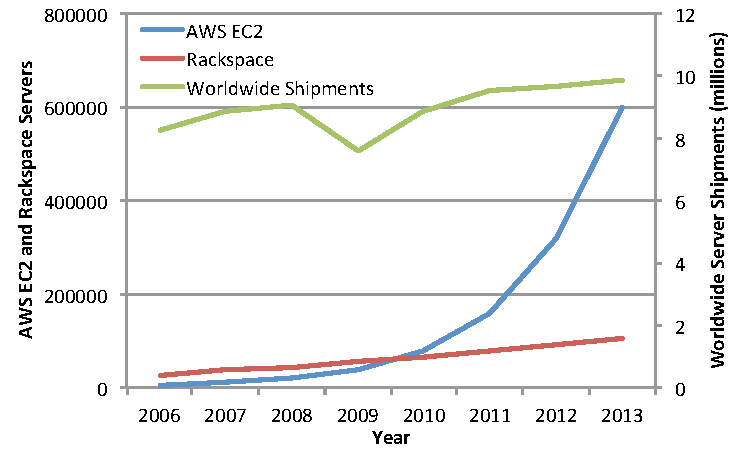
\includegraphics[height=3.5cm]{fig01}
\caption{Worldwide server shipments, Rackspace servers, and AWS EC2 servers}
\label{fig:servershipments}
\end{figure}

\subsection{Growth of Demand in Different Market Segments}
Figure \ref{fig:servershipments} shows the number of worldwide server shipments, the number of servers owned by Rackspace, and the estimated number of servers deployed for AWS EC2 between 2006 and 2013. As shown in Figure \ref{fig:servershipments}, the demand in server sales business is far greater than the demand in server rental business and public clouds. However, the server sales business and the server rental business exhibit close-to-linear growth, while the pubic cloud business exhibits exponential growth. In other words, the demand for public clouds is growing much faster than the demand for the other two business segments. 

\section{Analysis on Price Elasticity of Demand}
\label{sec:analysis}
In this section, we first introduce the microeconomics concept of price elasticity of demand, describe its application to the enterprise computing resource market. Then, we present our analysis on price elasticity of the three market segments.

\subsection{Price Elasticity of Demand}

To study how sensitive the consumers are to price changes, we borrow the concept of price elasticity of demand from microeconomics. Usually, price elasticity of demand is used to measure the consumer's sensitivity of price changes for a particular product. The enterprise computing resource market, however, includes many different products with dramatically different configurations such as CPU, memory, storage and networking. To apply this concept to the enterprise computing resource market, we make the assumption that the products being offered in each market segment are statistically the same, and can be treated as a homogeneous product sharing a common average unit price. With this approach, we can calculate the price elasticity of demand for a market segment using market research data on a macro scale, such as total server shipments and total revenue for the server sales business. The same method can also be applied to calculate the price elasticity of demand for a specific supplier.

Price elasticity of demand is defined by the percentage change in demand over the percentage change in price. More formally,
%The formula to calculate the price elasticity of demand is

\begin{equation}
E = \frac{\left ( \frac{dQ}{Q} \right )}{\left ( \frac{dP}{P} \right )} ,
\end{equation}
\\where $E$ represents the price elasticity of demand, $P$ represents the price and $Q$ represents the quantity sold, while $dP$ and $dQ$ represent the percentage changes (in absolute values) in price and demand. When $E$ is greater than 1, the percentage change in demand is greater than the percentage change in price, which is classified as elastic demand. When $E$ is smaller than 1, the percentage change in demand is smaller than the percentage change in price, which is classified as inelastic demand. When $E$ equals to 1, the percentage change in demand equals to the percentage change in price, which is classified as unitary demand. When demand is inelastic, a rise in price leads to a rise in revenue. When demand is elastic, a fall in price leads to a rise in revenue. 

To identify the price elasticity of demand in this study, we carry out linear regression with history price and demand data. With such a technique, we can express the relationship between price and demand as

\begin{equation}
Q = b_0 + b_1 P .
\end{equation}

The slope of a linear curve $b_1$ can also be expressed as

\begin{equation}
b_1 = \frac{dQ}{dP} .
\end{equation}

Therefore

\begin{equation}
\label{eq:elasticity}
E = - b_1  \frac{P}{Q} .
\end{equation}

For a particular product, the price elasticity of demand is not a constant. Rather, it is a variable closely related to both price and demand in a particular time frame. In general, there are two factors contributing to the price elasticity of demand. The first factor is the availability of close substitutes. If a buyer has greater choice among close substitutes in consumption, the price elasticity of demand is greater. The second factor is the proportion of a buyer's budget that is devoted to a product. The larger the proportion of budget, the more responsive is the quantity demanded to price changes, and the price elasticity of demand is greater.

\begin{figure}[t!]
\centering
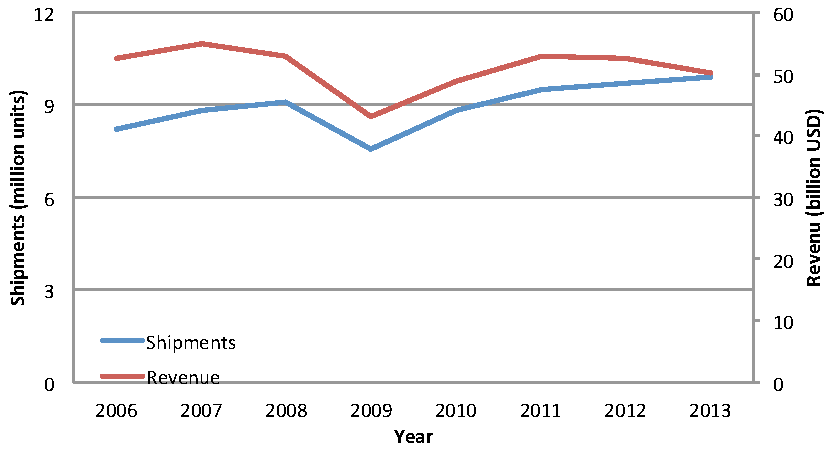
\includegraphics[height=3.5cm]{fig02}
\caption{Worldwide server shipments and total revenue}
\label{fig:shipmentsNrevenue}
\end{figure}

\begin{figure}[t!]
\centering
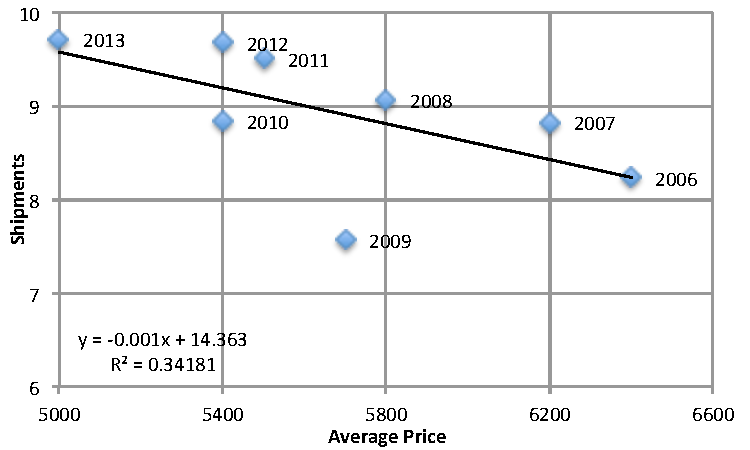
\includegraphics[height=3.5cm]{fig03}
\caption{Demand curve for server hardware}
\label{fig:shipmentsNunitprice}
\end{figure}


\subsection{Price Elasticity of Server Sales Business}
\label{sec:priceServerSales}

We plot the number of worldwide server shipments and the revenue generated by the server sales business between 2006 and 2013 in Figure \ref{fig:shipmentsNrevenue} and show the price elasticity of demand in Figure \ref{fig:shipmentsNunitprice}, respectively.
The significant drop in both server shipments and revenue in 2009 was the result of the global economic recession, which started in 2008 and ended in 2009. 
Figure \ref{fig:shipmentsNunitprice} is a supply and demand plot for the server sales business with a linear regression trend line. In the  supply and demand plot, supply is represented by the price, while demand is represented by the number of server shipments. %Each point (x, y) in the supply and demand plot represents the supply and demand relationship for a particular year, with x representing the average unit price and y representing the the number of server shipments. 
Using Equation \ref{eq:elasticity}, the price elasticity of demand for the worldwide server market is calculated as 0.51 in 2013; hence, it is extremely inelastic. The actual calculation is done with the slope of the trend line (-0.001), the number of worldwide server shipments (9.72 million) and an average unit price of 5000 USD.
%The slope of the trend line is -0.0001, while the number of worldwide server shipments is 9.72 million in 2013, with an average unit price of 5000 USD. Using Equation \ref{eq:elasticity}, we calculate that the price elasticity of demand for the worldwide server market is 0.51 in 2013 is extremely inelastic.  

For the majority of enterprise consumers, when they need computing resource the first option that comes to mind is purchasing some server hardware. Other forms of computing resource are not close substitutes for various reasons---renting server hardware from hosting service providers might pose security problems, while public clouds have not been widely adopted. From a budget perspective, server hardware purchases, as fixed-asset investments, are usually decided at the organization level, and are only a small proportion of an organization's annual budget. The lack of close substitutes, and the small proportion of budget, combined contribute to the inelastic demand in server hardware. In other words, organizations invest on server hardware based on their business plans, regardless of price changes in the market. 

A fundamental characteristic of inelastic demand is that the percentage change in demand is less than the percentage change in price. In this case, price reduction might produce more demand, but will also result in revenue lost. In a perfectly monopoly industry, the vendor would always do the opposite, i.e., raising the price and harvesting more revenue. The problem is, the competition in the server hardware market is extremely intensive. Leading server vendors are cutting prices to win market share. Regardless of the steady growth in worldwide server shipments, the overall revenue from server sales seems to be decreasing, as shown in Figure \ref{fig:shipmentsNrevenue}. This results in decreasing margin from server sales, and makes it difficult for server vendors to survive. 

\begin{figure}[t!]
\centering
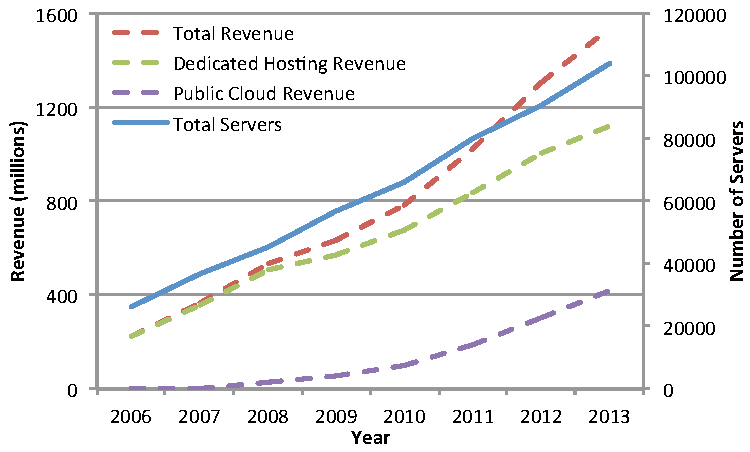
\includegraphics[height=3.5cm]{fig04}
\caption{Rackspace's servers and revenue}
\label{fig:rackspaceNrevenue}
\end{figure}

\begin{figure}[t!]
\centering
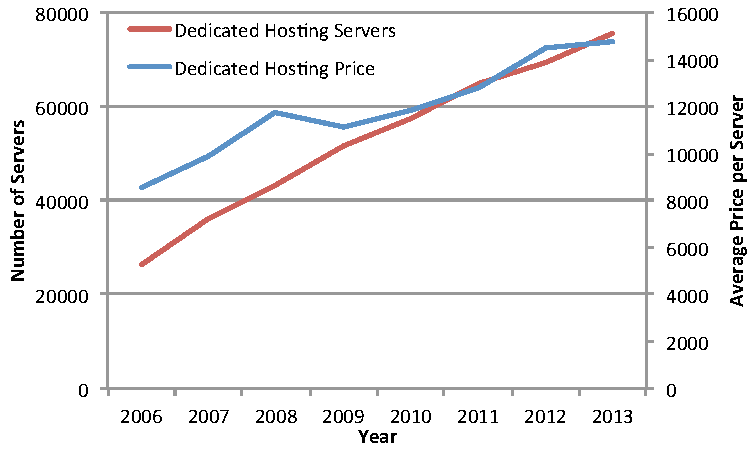
\includegraphics[height=3.5cm]{fig05}
\caption{Rackspace's servers and the average revenue per server}
\label{fig:rackspaceNavgrevenue}
\end{figure}


\subsection{Price Elasticity of Server Rental Business}

As Rackspace is a good representative in server rental business, we analyze the price elasticity of demand of Rackspace.
Figure \ref{fig:rackspaceNrevenue} shows Rackspace's number of servers and revenue, as well as the revenue break down for dedicated hosting (server rental business) and public cloud between 2006 and 2013. During this period, the number of servers is growing linearly, with an average of 11,000 new servers every year. Between 2006 and 2008, the revenue from dedicated hosting is growing at approximately the same rate as the growth in the number of servers, as reflected in the similar slopes of the two lines.  During this period, the revenue from its public cloud business is growing very slowly, and only represents less than 10\% of the total revenue. Since 2009, the revenue growth from dedicated hosting is slightly slower than it was before, while the revenue from the public cloud business is growing rapidly. In 2013, the revenue from the public cloud business contributes 27\% of Rackspace's total revenue.

To study the price elasticity of demand for the server rental market, we need to estimate the number of servers being used for dedicated hosting. In order to do so, we make two assumptions. The first assumption is the percentage of servers being deployed for each business is proportional to the revenue they bring in, but with different weights at different stages. The second assumption is that as the public cloud business continues to mature, its average revenue per server becomes higher than the average revenue per server from dedicated hosting (otherwise there is no incentive for hosting service providers to invest on cloud technologies). The increase in average revenue per server from public cloud is the result of increased resource efficiency introduced by virtualization and multi-tenancy. In this calculation, we assume that the average revenue per server from public cloud is the same as dedicated hosting between 2006 and 2008, but gradually grows in a linear fashion to 150\% of the average revenue per server from dedicated hosting from 2009 to 2013. The above-mentioned 150\% is derived from the ratio between the overall average revenue per server in 2013 and 2006, which is 173\%.

Figure \ref{fig:rackspaceNavgrevenue} shows the estimated number of servers and the estimated average revenue per server for Rackspace's dedicated hosting business. The number of servers is growing linearly, with about 7,000 new servers every year. The average revenue per server also exhibited near-linear growth, with an exception in 2009, which was the result of the global economic recession between 2008 and 2009. In general, we are observing a strong growth in demand together with a strong growth in price. It should be noted that the number of worldwide server shipments discussed in Section \ref{sec:priceServerSales} represents the newly added computing resource every year. Further more, the life cycle of server hardware is usually more than one year, and in most cases falls within the range of three to five years. The number of servers for Rackspace's dedicated hosting business represents the accumulated computing resource over the past years. To facilitate a fair comparison, we calculate the annual server increments for Rackspace's dedicated hosting business, and use that number to compare with the server sales business. Figure \ref{fig:demandRackspace} is a supply and demand plot with the average revenue per server on the horizontal axis and the annual server increments on the vertical axis, with a linear regression trend line. The calculated price elasticity of demand for Rackspace's dedicated hosting business is 0.70 in 2013, which is modestly inelastic.

Enterprise consumers choose server rental over buying server hardware for various reasons. For small and medium businesses, the cost and effort to build and maintain a small data center with the appropriate networking capacity is overwhelming. There are many server hosting service providers available, including international and local ones. An enterprise usually needs to go through a comparison and selection process before deciding which one to work with. Once a decision has been made, a long-term contract with the selected service provider will be setup. The length of such contract is usually measured by months or even years, depending on the consumer's business plan. Such a long-term contract effectively eliminates the possibility of migrating to alternative options when there is a price change in the market. Thus, enterprise consumers invest on server rental based on business plans, which are usually not sensitive to price changes. This is why the price elasticity of demand for the server rental business is inelastic. 

\begin{figure}[t!]
\centering
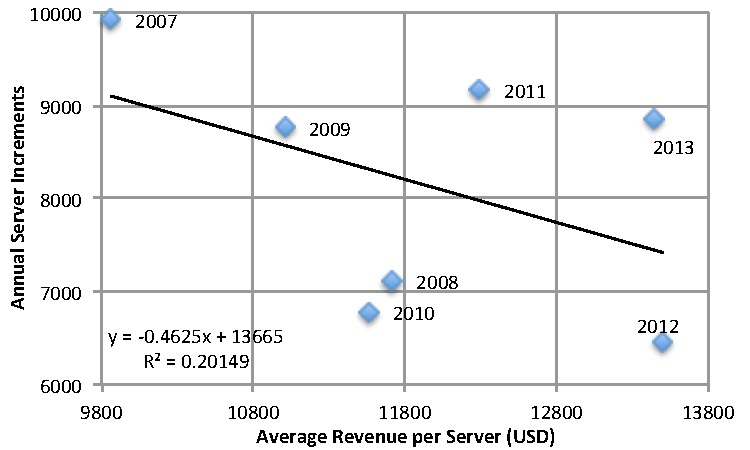
\includegraphics[height=3.5cm]{fig06}
\caption{Demand curve for Rackspace's dedicated hosting business}
\label{fig:demandRackspace}
\end{figure}

\begin{figure}[t!]
\centering
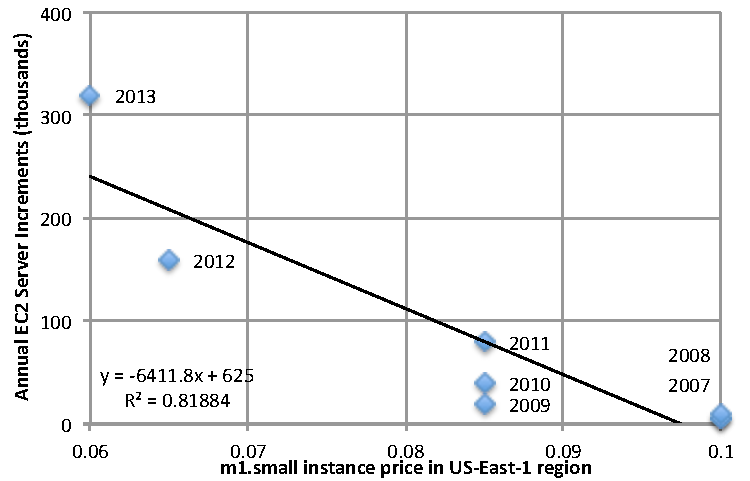
\includegraphics[height=3.5cm]{fig07}
\caption{Demand curve for Amazon EC2 Service}
\label{fig:demandEC2}
\end{figure}


\subsection{Price Elasticity of Public Clouds}

The lack of published data makes it difficult to carry out a similar analysis for AWS EC2. We notice that the US-East-1 region is the largest EC2 region, which accounts for approximately one half of all EC2 usages. Also, the first generation standard instance types (the m1 instances family) are the most commonly used instance types on EC2, and the prices for these instance types are approximately proportional to their configurations. Therefore, we estimate the price elasticity of demand for EC2 with the assumptions that (a) the on-demand price of the m1.small instance type in the US-East-1 region represents the price of EC2 instances; and (b) the EC2 data centers are being utilized in a highly efficient way that the amount of servers is a direct indicator of demand for EC2 instances. Similar to the analysis for the server rental market, we are more interested in the demand for new computing resource represented by the annual increments in EC2 servers, rather than the accumulated total demand represented by the total number of EC2 servers. Figure \ref{fig:demandEC2} is a supply and demand plot showing the estimated amount of annual EC2 server increments and the price of m1.small instance in US-East-1 region between 2008 and 2013, with a linear regression trend line. The calculated price elasticity of demand is 1.20 in 2013, which is modestly elastic.

Many consumers consider EC2 as an alternative to traditional server rental services and virtual private server (VPS) services, while ignoring those advanced features such as CloudWatch, AutoScaling, and Elastic Load Balancing. Furthermore, spending on EC2, as an operations expense, is usually decided at the project level, and is usually a big portion of a project's budget. The availability of close substitutes, and the big proportion of budget, combined contribute to the elastic demand for EC2. In other words, enterprise consumers spend on EC2 based on actual business needs rather than business plan, and are sensitive to price changes because of budget limitations.

In general, inelastic demand is closely related to planned buying, while elastic demand is closely related to unplanned buying. With the fixed-asset model, when enterprise consumers need computing resource, the budget for the needed computing resource must first be secured before making an order. Then it takes weeks, if not months, for the needed computing resource to be delivered and deployed. With the utility model, consumers have instant access to computing resource with no capital expense, zero lead time, at affordable prices. In other words, the utility model makes it possible for customers with a limited budget to do big things. This applies to both general purpose enterprise computing as well as complex science, engineering, and business problems requiring high bandwidth, low latency networking, and very high compute capabilities. With AWS, customers can even build supercomputers that matches the capability of top 100 performing supercomputers in the world\cite{top500}.\footnote{A compelling example is Cycle Computing's record-setting cloud computing deployment of a 16,788 Amazon EC2 instance cluster with 156,314 cores across 8 regions for materials science experiments that screen 205k candidate molecules (\url{http://tinyurl.com/o6sz969 }.} Such a model becomes a catalyst for innovations that generate additional demand for computing resource. For example, George et al. \cite{jpl} reported that NASA's Jet Propulsion Laboratory (JPL) utilized the AWS services to broadcast the landing event of the Curiosity Mars Rover in real time to a global audience. The broadcasting event was not part of JPL's Mars exploration research plan, and could in no way be satisfied with NASA's own infrastructure. In fact, such a broadcasting event would not have come to NASA's consideration if AWS services were not available. 

\section{Case Studies}
\label{sec:casestudies}

\begin{figure}[t!]
\centering
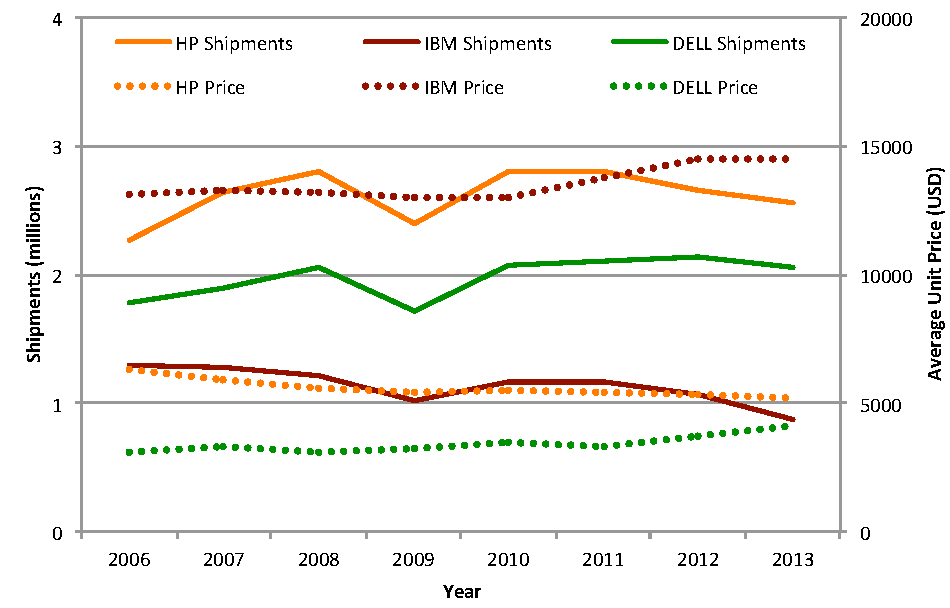
\includegraphics[height=4.0cm]{fig08}
\caption{Server shipments and average prices for HP, IBM, and DELL}
\label{fig:shipmentsHPIBMDELL}
\end{figure}

\begin{figure}[t!]
\centering
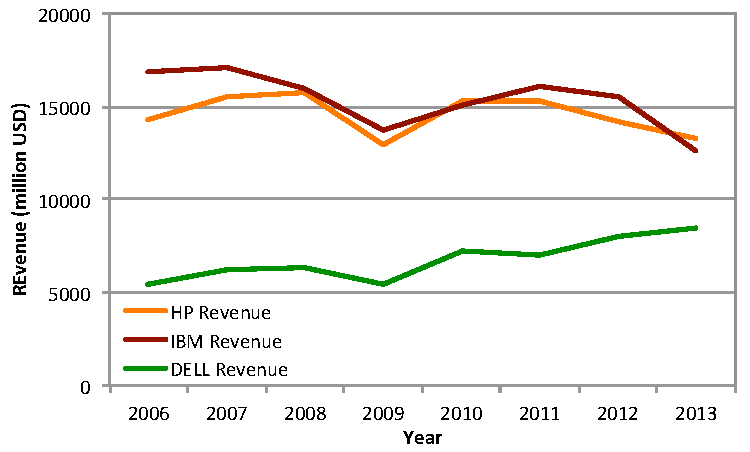
\includegraphics[height=3.5cm]{fig09}
\caption{Revenue for HP, IBM, and DELL}
\label{fig:revenueHPIBMDELL}
\end{figure}


In this section, we analyze the impact of different pricing strategies on the performance of the business, using IBM, HP and DELL as case studies.  

Figure \ref{fig:shipmentsHPIBMDELL} shows the annual server shipments and the average prices for IBM, HP and DELL. The significant gaps in the average prices indicate that these vendors are not competing in the same fine-grained market segment. IBM dominates the high-end server market with an average price above 13,000 USD, HP occupies the mid-range server market with an average price around 6,000 USD, while DELL dominates the low-end server market with an average price below 4,000 USD (see market research data accumulated in \cite{qyjohn} for details). 

For IBM, the average price does not change much between 2006 and 2010. The slight decrease in its annual server shipments during this period is not a response to price adjustments. Rather, it is an indicator that the market preference is gradually shifting from high-end servers to mid-range and low-end servers. The global economic recession between 2008 and 2009 is also accountable for the reduction in server shipments. Between 2010 and 2012, there is an 11\% increase in IBM's average price, with a corresponding 8\% decrease in server shipments. During this period, the price elasticity of demand for IBM servers is 0.73, which is modestly inelastic.\footnote{We intentionally ignore data in 2013, because IBM sold its server business to Lenovo in Jan. 2014 (http://tinyurl.com/qdm2svg).} For HP, there is an 18\% percent decrease in average price between 2006 and 2013, with a corresponding 13\% increase in server shipments. During this period, the price elasticity of demand for HP servers is 0.72, which is very similar to IBM. For DELL, there is a 28\% increase in average price, with a corresponding 15\% increase in server shipments. The simultaneous increase in price and shipments indicates that the price elasticity of demand for DELL servers is extremely inelastic - the demand increases regardless of price increases. 

As we can see, the price elasticity of demand for IBM, HP and DELL servers are inelastic. The in-elasticity in demand, plus the significant gaps in the average prices, suggest that enterprise consumers do not perceive IBM, HP and DELL servers as close substitutes for each other. These vendors are de-facto monopolies in their own fine-grained market segment, and have the market power over pricing. The market preferences, as well as their own pricing strategies, contribute more to the changes in revenue (Figure \ref{fig:revenueHPIBMDELL}) than the impact from competitors. IBM decides to increase the average price, which is a favorable response to inelastic demand. However, the market preference is shifting from high-end servers to mid-range and low-end servers, resulting in the decrease in revenue from IBM's server business. Such a shift in market preferences is probably the primary reason IBM sold its server business to Lenovo in January 2014. HP decides to decrease the average price, which is an unfavorable response to inelastic demand. This leads to an increase in server shipments, along with a decrease in revenue. DELL decides to increase the average price, which is a favorable response to inelastic demand. Coupled with the shift in market preference from high-end servers to mid-range and low-end servers, DELL achieves a simultaneous increase in server shipments and revenue. 

\section{Related Work}
\label{sec:relatedwork}

Chow \cite{chow} studies the technological change and the demand for computers with the price and quantity of computers in the United States between 1955 and 1965. He indicates that two elements account for the natural increase in the use of computers: (a) it takes time for a new product to reach an equilibrium level; and (b) the quality of the product is improving, so that the equilibrium level is being continuously raised. He also concludes that the Gompertz differential equation, modified by a moving equilibrium, matches best with the rate of growth for this new commodity. Tam et al. \cite{tam} extend Chow's work with annual computer hardware spending data in the United States between 1955 and 1984. Their findings indicate that the price elasticity of demand for computer hardware is inelastic, but the degree of elasticity changes over time. The data sources being used in \cite{chow} are \cite{tam} are extremely old, while technology advancements have dramatically changed the horizon of the computing resource market in general. These changes not only change the demand for computing resource, but also the relationship between supply and demand. 

Stavins \cite{stavins} studies the price elasticity of demand for the personal computer market with annual personal computer sales data in the United States between 1976 and 1988. He identifies that the prices elasticity of demand varies across computer models according to their market power. In general, the price elasticity of demand increases over time, while the brand effect on the market share of a particular model declines. Goolsbee \cite{goolsbee} compares the price sensitivity on computer purchases from online stores versus in retail stores, and identifies that customers are more sensitive to price changes when they are shopping online. 

Yeo et al. \cite{yeo} analyze the pros and cons of charging fixed prices as compared to variable prices for utility computing services, and proposes a pricing mechanism capable of achieving higher revenue than fixed pricing and other variable pricing mechanisms. Paleologo \cite{paleologo} considers the uncertainty in demand for utility computing services, and proposes a ``price-at-risk'' method to optimize the ``net present value'' of utility computing services. Durkee \cite{durkee} studies the behavior of virtual private server (VPS) service providers who try to maintain both low pricing and profitability. He points out that the pricing wars result in products that do not meet enterprise requirements, and threaten the long-term viability of cloud service providers. 

Brynjolfsson et al. \cite{erik} discuss the strength and weakness of the utility model, and compare cloud computing with the electricity industry. They point out that there exist significant technical differences, as well as differences in business model, between cloud computing and the electricity industry. They conclude that cloud computing is a catalyst for more innovation, especially when it continues to become cheaper and more ubiquitous. 

\section{Conclusions}
\label{sec:conclusions}

In the paper, we study the relationship between price and the amount of computing resources sold on the global enterprise computing resource market, using market research data between 2006 and 2013. We reveal and conclude that:


1. The enterprise computing resource market is not a perfect competition market. In the server sales business, the significant gaps in their average unit prices indicate that the hardware vendors are not competing in the same fine-grained market segment. IBM dominates the high-end server market, HP occupies the mid-range server market, while DELL dominates the low-end server market. They are de-facto monopolies in their own fine-grained market segment, and have the market power over pricing.


2. With the assumption that computing resources are statistically homogeneous, the concept of price elasticity of demand can be used to measure the consumer's sensitivity to price changes for a market segment as well as a particular supplier. The price elasticity of demand is extremely inelastic for the server sales business. This indicates that enterprise customers purchase server hardware based on their business plan and are less sensitive to price changes in the market. The price elasticity of demand is modestly inelastic for the server rental business. Enterprise consumers renting servers from hosting service providers are more sensitive to price changes than enterprise consumers buying server hardware. However, they are not able to response to price changes in the market due to existing contracts. The price elasticity of demand is modestly elastic for public clouds. This indicates that enterprise consumers using public cloud are sensitive to price changes, and tend to respond to price deductions with increasing consumption.

3. For market segments with inelastic demand, price reduction is not an effective way to win market share. For market segments with elastic demand, price reduction is an effective way for market diffusion. In our case studies, IBM makes a favorable response to the inelastic demand by raising the price, but the market preference is migrating from high-end servers to mid-range and low-end servers, resulting in decreases in both server shipments and revenue. HP makes an unfavorable response to the inelastic demand by lowering the price, resulting in increases in server shipments but decreases in revenue. DELL makes a favorable response to the inelastic demand by raising the price, resulting in increases in both server shipments and revenue.

This paper provides new insights into the microeconomics characteristics of the enterprise computing resource market. It represents the state of the art on the relationship between supply and demand, and forms the foundation for further researches on competition and pricing strategies in the enterprise computing resource market. 

\bibliographystyle{ieeetr}  
\bibliography{mybibfile_small}

\begin{IEEEbiographynophoto}{Qingye Jiang}
is pursuing his Master of Phisolophy degree in the School of Information Technologies at The University of Sydney. His research interests include open source communitites, the economics of cloud computing, cloud interoperability, as well as the quality, availability and reliability of cloud service. He is a senior member of IEEE.
\end{IEEEbiographynophoto}

\begin{IEEEbiographynophoto}{Young Choon Lee}
is with the Centre of Parallel and High Performance Computing in the School of Information Technologies at The University of Sydney.
\end{IEEEbiographynophoto}

\begin{IEEEbiographynophoto}{Albert Y. Zomaya}
is currently the chair professor of high performance computing and networking in the School of Information Technologies, The University of Sydney. He is the author/coauthor of seven books, more than 400 papers, and the editor of nine books and 11 conference proceedings. He is a fellow of IEEE, IET, and AAAS.
\end{IEEEbiographynophoto}

\end{document}